% \documentclass[conference]{IEEEtran}
\documentclass[twocolumn]{IEEEtran}
\usepackage[compatibility=false]{caption}
\usepackage{subcaption}
\usepackage{booktabs}
\IEEEoverridecommandlockouts
\usepackage{cite}
\usepackage{amsmath,amssymb,amsfonts,esint}
\DeclareMathOperator{\sinc}{sinc}
% \usepackage{algorithmic}  % unused; requires texlive-science
\usepackage{graphicx}
\usepackage{textcomp}
\usepackage{xcolor}
\usepackage{hyperref}

\def\BibTeX{{\rm B\kern-.05em{\sc i\kern-.025em b}\kern-.08em
    T\kern-.1667em\lower.7ex\hbox{E}\kern-.125emX}}
    
\begin{document}

\title{Open-Source SAR Simulator in PyTorch Via Interposummation
\thanks{This work was supported by STR (under a contract with DARPA) and Arete (with STTR research funding).\\Code: \href{https://github.com/alexberian/PyTorch-SAR-SONAR/}{https://github.com/alexberian/PyTorch-SAR-SONAR/}}
}

\author{
\IEEEauthorblockN{Alex Berian, Sehajdeep Singh Bal, JhihYang Wu, Daniel Brignac, Abhijit Mahalanobis}
\IEEEauthorblockA{
\textit{Department of Electrical and Computer Engineering} \\
\textit{The University of Arizona} \\
Tucson, AZ, USA \\
berian, sehajdeepbal, jhihyangwu, dbrignac, amahalan@arizona.edu
}
}

\maketitle

\begin{abstract}
There is currently a lack of open-source SAR simulators. \emph{RaySAR} supports only stripmap-mode
imaging and ignores multi-bounce ray interactions, while \emph{CVDomes} is limited to a few CAD
models and spotlight mode. Both depend on outdated software such as MATLAB and POV-Ray.
We present an \emph{open-source SAR simulator} implemented in \emph{PyTorch} with \emph{GPU
acceleration}. It supports arbitrary \texttt{.obj} 3D models, with configurable wavelength, sample
rate, radar pulse bandwidth, and material properties. It simulates the recovered signal from a
range of azimuth and elevation angles, supporting applications such as stripmap- and
spotlight-mode imaging, radar cross section modeling, simulating different noise types, jamming,
and imperfect sensor trajectories. We simulate multi-bounce ray tracing to model realistic
reflectivity, scattering, and absorption.

We introduce an efficient low-pass filtering technique for summation and interpolation of ray
returns, termed \emph{interposummation}. Interposummation accounts for the effective bandwidth and
sample rate of the radar system. We test our simulator on ShapeNet car models with spotlight-mode
imaging.\end{abstract}

\begin{IEEEkeywords}
SAR, Radar, Ray Tracing, Simulator
\end{IEEEkeywords}

\section{Introduction}
\label{sec:intro}

\begin{figure}[t]
    \centering
    % Row 1
    \begin{subfigure}{0.2\textwidth}
        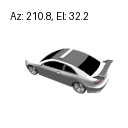
\includegraphics[width=\linewidth]{figs/rgb.png}
        \caption{}
    \end{subfigure}
    \hfill
    \begin{subfigure}{0.2\textwidth}
        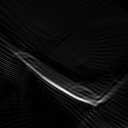
\includegraphics[width=\linewidth]{figs/sar.png}
        \caption{}
    \end{subfigure}

    % Row 2
    \begin{subfigure}{0.2\textwidth}
        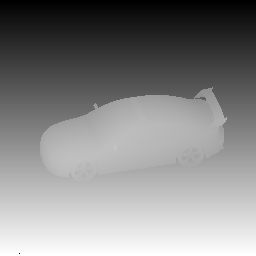
\includegraphics[width=\linewidth]{figs/depth-map.png}
        \caption{}
    \end{subfigure}
    \hfill
    \begin{subfigure}{0.2\textwidth}
        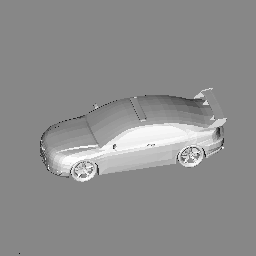
\includegraphics[width=\linewidth]{figs/energy-map.png}
        \caption{}
    \end{subfigure}

    % Row 3
    \begin{subfigure}{0.2\textwidth}
        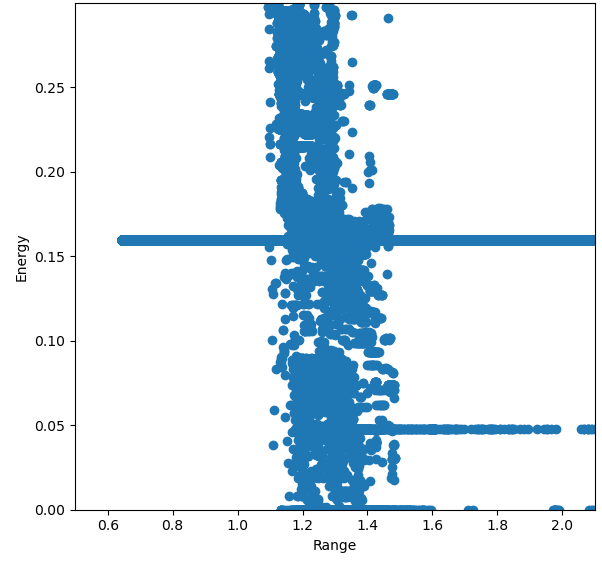
\includegraphics[width=\linewidth]{figs/scatters.png}
        \caption{}
    \end{subfigure}
    \hfill
    \begin{subfigure}{0.2\textwidth}
        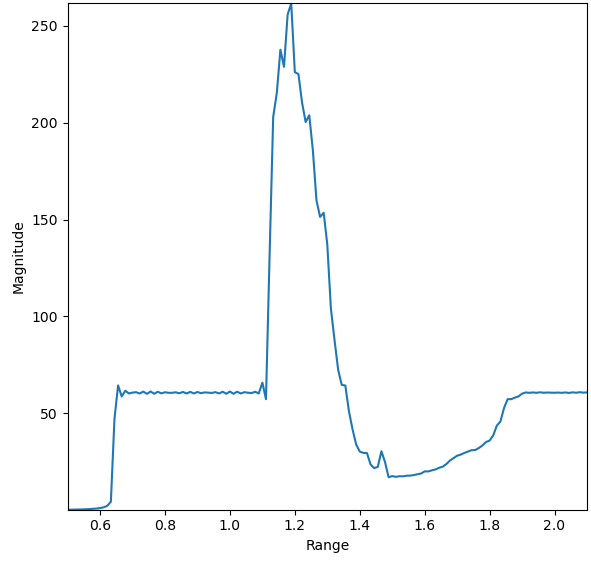
\includegraphics[width=\linewidth]{figs/signal_clean.png}
        \caption{}
    \end{subfigure}

    \caption{Example of the simulation. (a) RGB image of the ShapeNet \cite{shapenet} car model, (b) spotlight-mode SAR image of the model from our simulation, (c) range per ray, (d) returned energy per ray, (e) energy-range scatter, (f) signal calculated via interposummation.}
    \label{fig:main-fig}
\end{figure}

\begin{figure}[t]
    \centering
    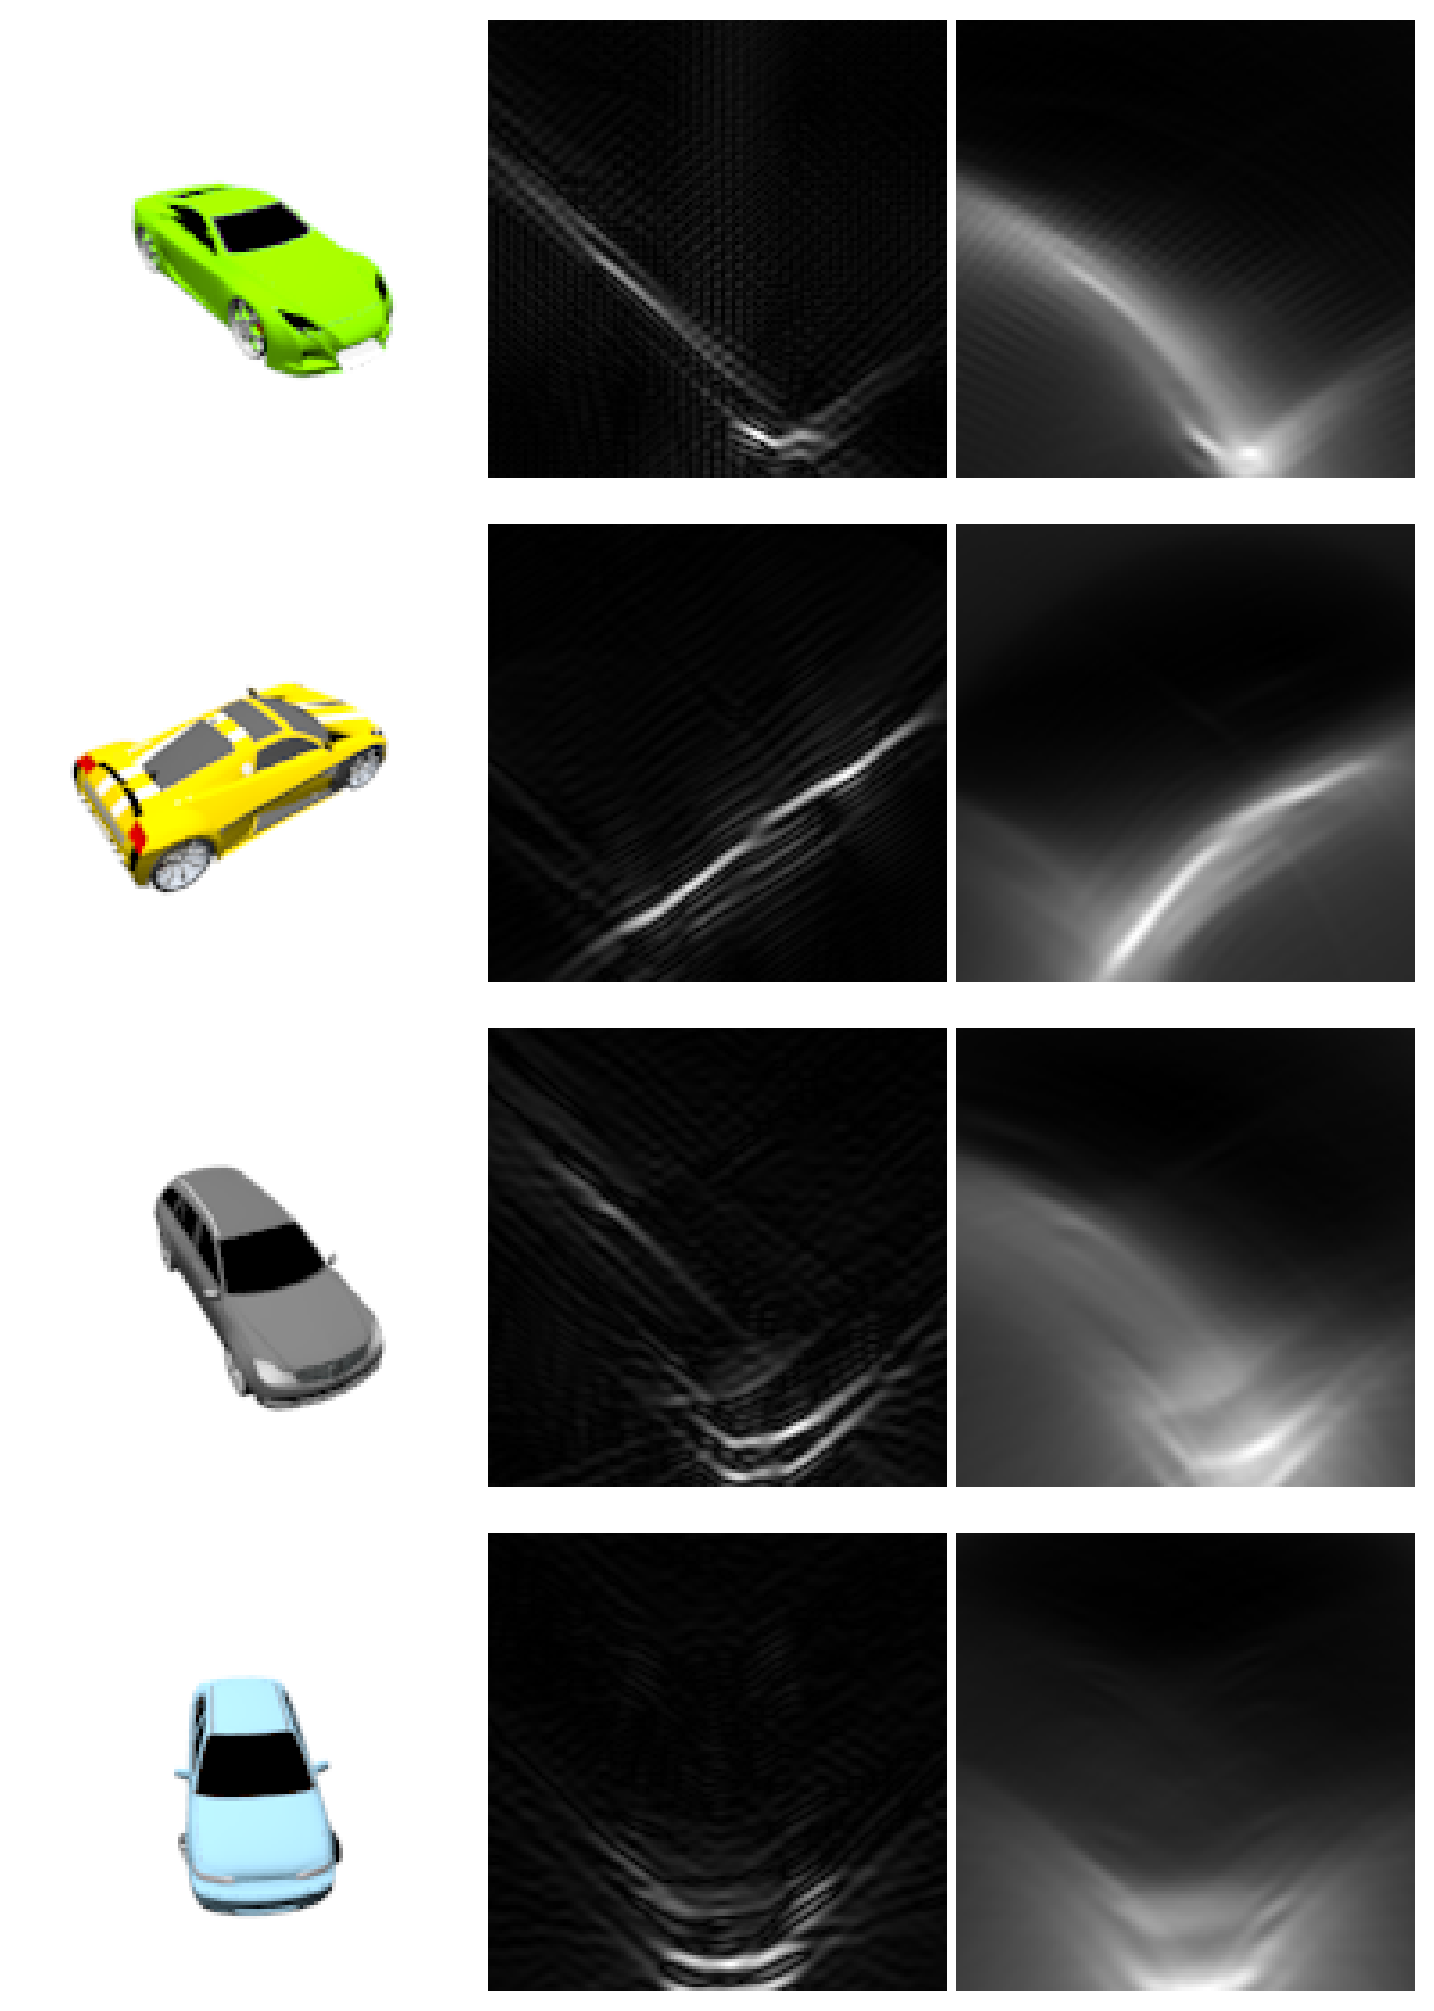
\includegraphics[width=0.95\linewidth]{figs/linear_sar_comparison.png}
    \par\vspace{2pt}
    \makebox[0.95\linewidth]{%
        \makebox[0.3167\linewidth]{(a)}\hfill
        \makebox[0.3167\linewidth]{(b)}\hfill
        \makebox[0.3167\linewidth]{(c)}%
    }
    \caption{Both spotlight-mode and stripmap-mode imaging from the same simulated signals for four ShapeNet \cite{shapenet} car models. (a) RGB image of each model, (b) spotlight-mode SAR image, and (c) stripmap-mode SAR image.}
    \label{fig:linear-sar}
\end{figure}

\begin{figure*}
  \centering
  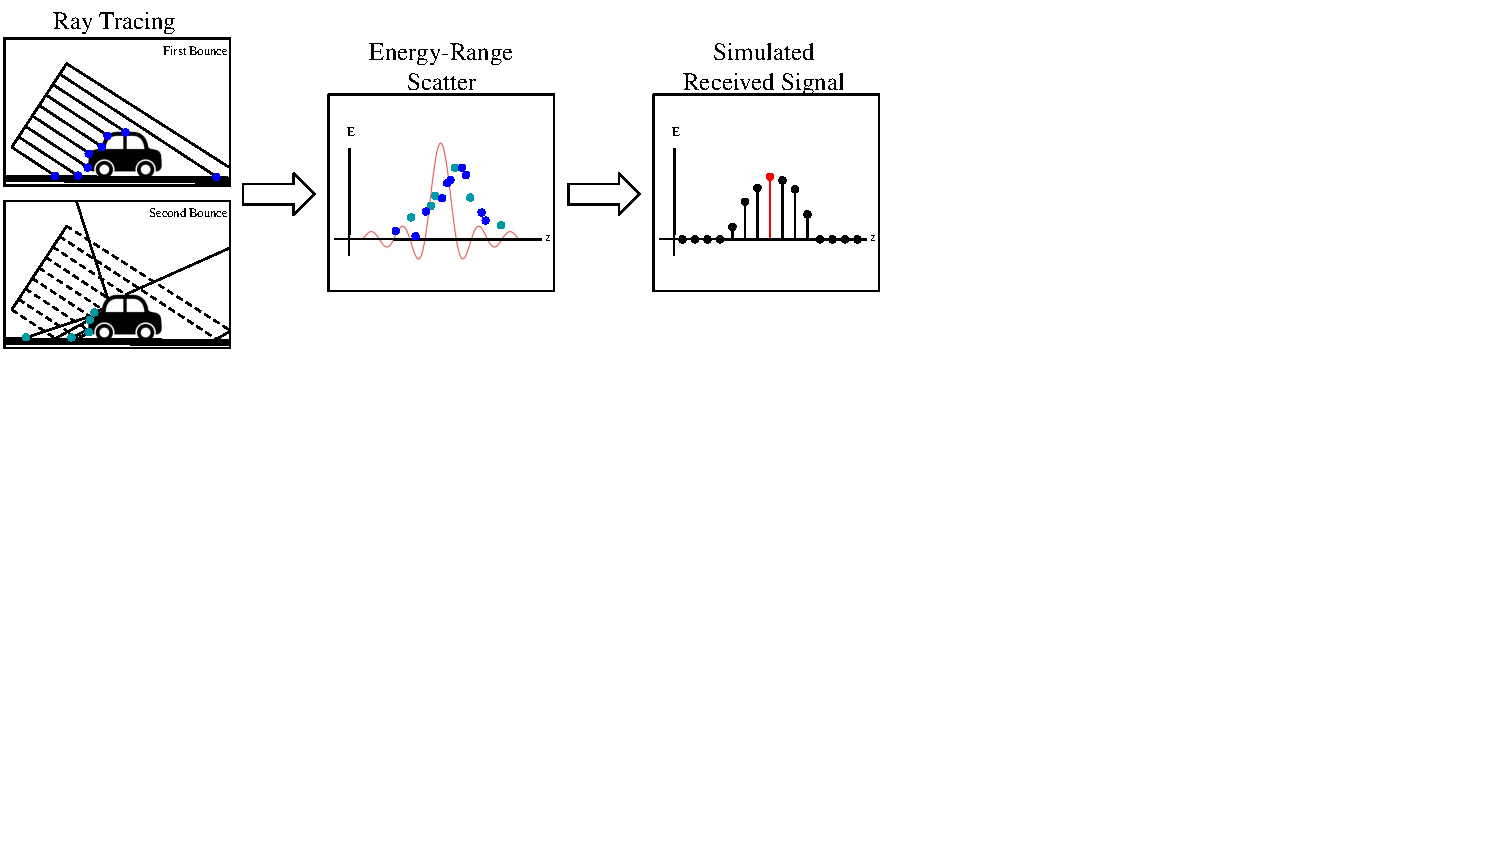
\includegraphics[trim=0 241 289 0, clip, width=0.8\textwidth]{figs/ray-trace-sim.pdf}
  \caption{Process for simulating the received signal from object meshes.}
  \label{fig:sig-sim}
\end{figure*}

SAR simulators are crucial for developing and validating radar algorithms when real-world data is unavailable or not feasible to process. By providing controlled, repeatable environments, simulators allow researchers to test imaging techniques, evaluate performance under different conditions, and benchmark novel methods without requiring extensive field experiments.

Most powerful simulators, such as XPatch \cite{xpatch4}, are either classified in some manner or proprietary to their respective developer. Open-source simulators like CVDomes \cite{cvdomes} and RaySAR \cite{raysar} lack flexibility and rely on outdated software.

To the best of our knowledge, we provide the first scalable PyTorch-based SAR simulation framework that allows for any 3D \texttt{.obj} model. Our simulator allows users to specify sample rate, bandwidth, material properties (reflectivity, scatter, absorption), and sensor trajectory.
The primary functionality of the simulator is to use ray tracing combined with an interpolation/summation technique we call \emph{interposummation} to simulate signals that correspond to the radar system's wavelength, bandwidth, and sample rate. We use two bounces from each ray. Given signals collected over a range of azimuth and elevation angles, imaging algorithms such as spotlight-mode \cite{spotlightmodesar} or stripmap-mode SAR can be used. Figure \ref{fig:linear-sar} highlights this flexibility, reconstructing both spotlight-mode and stripmap-mode SAR images from the same set of simulated signals for four different ShapeNet car models.

Figure \ref{fig:main-fig} showcases an example of our simulator on a ShapeNet \cite{shapenet} car
model. The spotlight-mode SAR image is shown in Figure \ref{fig:main-fig}.b with a mean azimuth
angle of $210.8^\circ$ and a fixed elevation angle of $32.2^\circ$. Figures
\ref{fig:main-fig}.(c,d,e,f) are examples from just one pulse, but to construct the SAR image we
aggregate $30$ pulses over a $90^\circ$ azimuth angle spread. The depth (Figure
\ref{fig:main-fig}.c) and energy (Figure \ref{fig:main-fig}.d) maps shown are only for the first
bounce of each ray; the actual simulation uses $2$ bounces for realism.
The overall process of our signal simulation is shown in Figure \ref{fig:sig-sim}. Our simulation
functions by simulating a grid of parallel rays with equal energy. The rays hit a triangle on the
\texttt{.obj} mesh. When a ray hits the mesh, some of the energy is reflected, some energy is
scattered back to the sensor, and some energy is lost to absorption. The reflected energy is part
of a second bounce ray that once again hits another triangle on the mesh with reflectivity,
scattering, and absorption. We gather scattered energy (Figure \ref{fig:main-fig}.d) and its
corresponding traveled range (Figure \ref{fig:main-fig}.c) into an energy-range scatter plot
(Figure \ref{fig:main-fig}.e). From the energy-range scatter plot we use a sinc pulse, with width
corresponding to the radar system bandwidth, to sum and interpolate (interposummation) the
scatters into a single sample of the received signal (Figure \ref{fig:main-fig}.f). The spacing
between each sinc pulse corresponds to the sample rate of the radar system. Once there is a
received signal for each pulse at different azimuth and elevation angles, further analysis or
imaging (Figure \ref{fig:main-fig}.b) can be done.

\section{Related Works}
\label{sec:related}

To the best of our knowledge, there are only two other publicly available SAR data simulators.
RaySAR \cite{raysar} is a MATLAB repository for simulating stripmap-mode SAR images via ray
tracing. CVDomes \cite{cvdomes} is a MATLAB repository that simulates spotlight-mode SAR images
from a small set of CAD models.

\subsection{CVDomes}
\label{sec:cvdomes}

CVDomes is a physics-calibrated pipeline where facet CADs are augmented with an explicit asphalt
ground plane and per-facet material labels (PEC, absorber, glass, plastic, asphalt). Monostatic
scattering is computed with a high-frequency SBR front end followed by a physical-optics
surface-current integral. Sampling is co-designed in both frequency and angle. In frequency, 512
bins span a bandwidth of $5.35$ GHz about a center frequency of $9.6$ GHz. In angle, azimuth is
computed in $0.5^\circ$ sectors, each extrapolated by $\pm 0.25^\circ$, to yield an effective step
of $0.0625^\circ$. The result is a dome-wide phase history covering $360^\circ$ of azimuth and
$30^\circ$--$60^\circ$ of elevation, exported as MATLAB ``data domes'' with fully polarimetric
channels (HH, HV, VV) for downstream imaging.

\begin{figure}[t]
  \centering
  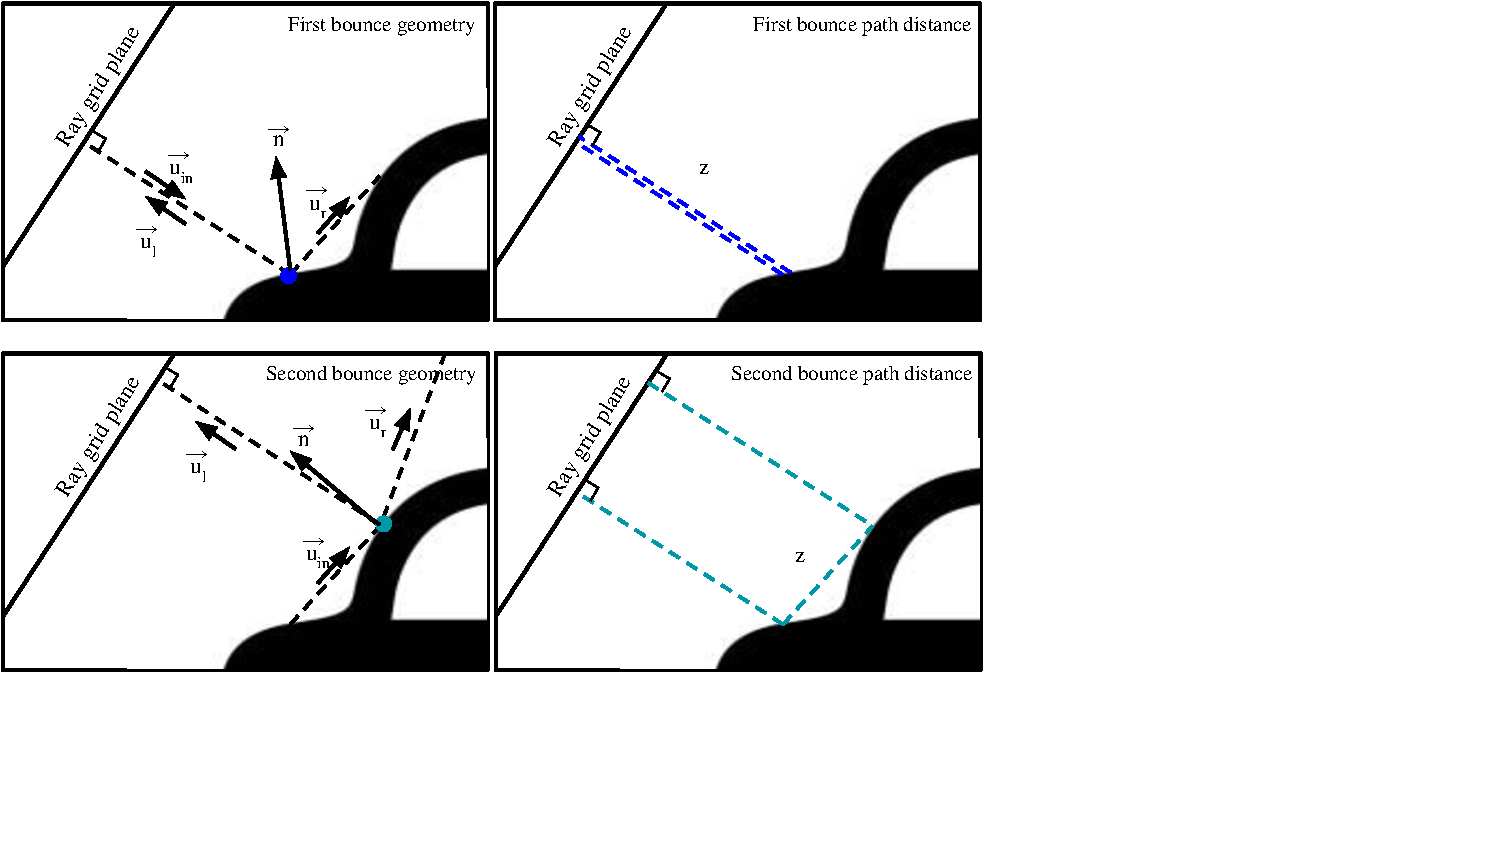
\includegraphics[trim=0 80 246 0, clip, width=\linewidth]{figs/terminology.pdf}
  \caption{Visual example of terminology for (\ref{eq:returned-energy}).}
  \label{fig:terminology}
\end{figure}


\subsection{RaySAR}
\label{sec:raysar}

RaySAR \cite{raysar} is a 3D SAR simulation tool that generates SAR-like images from detailed 3D
object models. The framework is built on a modified version of the POV-Ray tracer, using it to
simulate interactions between electromagnetic waves and surfaces of objects. Instead of
transmitting pulses or collecting real echoes, RaySAR performs geometric ray tracing to determine
which surfaces are illuminated, and estimates the backscatter of each surface from its local
incidence geometry relative to the radar sensor. This simulated backscatter is then projected into
the SAR slant-range coordinate system, producing radar-like images that capture geometric effects
such as layover, shadowing, and foreshortening. Users can define synthetic flight paths and
viewing geometries \cite{drozdowicz2021open} to analyze how different radar positions influence
the resulting image. RaySAR is therefore a forward-modeling tool: it predicts how 3D scenes would
appear in SAR imagery rather than simulating raw signal acquisition.

\section{Problem Statement}
\label{sec:problem}
A \texttt{.obj} file is a collection of $V$ vertices in 3D space and $F$ triangle faces. Our goal
is to produce a SAR/SONAR image from $P$ pulses. A signal needs to be simulated for each pulse
from a known azimuth angle $a$ and elevation angle $e$. From the simulated signals, we can do
further processing to produce SAR images or other analyses.

\section{Method}
\label{sec:method}

\subsection{Signal Simulation}


The general process for simulating signals is shown in Figure \ref{fig:sig-sim}. We cast a grid of
$R_h \times R_w$ parallel rays that originate on a grid of size $W_g \times H_g$. The center of the
grid intersects a line from the origin for a given azimuth $a$ and elevation $e$ angle. 
Azimuth $a$ is defined as the angle from the $x$ to the $y$ axis, and elevation $e$ is the 
angle from the $x$-$y$ plane to the $z$ axis. The grid is orthogonal to this line defined by the 
azimuth/elevation. This set of rays can be viewed as a simulated wavefront. The size of the ray 
grid only needs to be big enough to cover the ground space desired for imaging.

When a ray makes contact with a surface, some of the energy is reflected, some is absorbed, and 
some is scattered. We propose to model these three components as $R,S,A$. 
The scattering component is the only component where some of the energy comes back to the 
receiver. $R,S,A$ components are assigned to all $F$ faces in the object mesh. Metal surfaces have 
low scattering $S$ and absorption $A$, but high reflectivity $R$. In contrast, ground clutter 
tends to have high scattering and absorption.

Reflectivity, scattering, and absorption components of a particular part of the mesh should add up 
to 1 to ensure law of conservation of energy.
\begin{equation}
    R+S+A = 1
\end{equation}
Only scattering is considered for returned energy. Scattering occurs in two main ways: directional 
intensity $I$ and diffuse scattering $D$. To satisfy the law of conservation of energy, once again 
the components must add up to 1.
\begin{equation}
    D + I = 1
\end{equation}
Returned energy from a particular ray $E_r$ is given by
\begin{equation}
    E_r = E_{in} S \Big(m_I\cos({\theta/2})^\alpha + m_D\Big)
\end{equation}
where $E_{in}$ is the ray energy going into the surface, $\theta$ is the angle between the 
direction of the reflected ray $\vec{u}_r$ and the direction to the line of sight $\vec{u}_l$, and 
$m_I,m_D$ are multipliers to ensure law of conservation of energy is preserved.

We solve for the multipliers by ensuring that energy scattered in all directions integrates to
$SE_{in}$:
\begin{equation}
	S E_{in} = \oiint\limits_{H} S E_{in} \Big(m_I\cos({\theta/2})^\alpha + m_D\Big)d\Omega
\end{equation}
where $H$ denotes the hemisphere of directions from the surface.

\begin{equation}
    1 = m_I \oiint\limits_{H} \cos({\theta/2})^\alpha d \Omega + m_D \oiint\limits_{H} 1 d \Omega
\end{equation}

Now we can accurately ensure that the total amount of energy diffuse scattered is $D$ and the 
total amount of energy directionally scattered is $I$.
\begin{equation}
    \label{eq:directional-int}
    I = m_I \oiint\limits_{H} \cos({\theta/2})^\alpha d \Omega
    .
\end{equation}
\begin{equation}
    D =  m_D \oiint\limits_{H} 1 d \Omega = 2 \pi m_D
    .
\end{equation}

Using the half angle trigonometry identity,
\begin{equation}
    \cos\frac{\theta}{2} = \sqrt{\frac{1+\cos \theta}{2}}
    ,
\end{equation}
and we can express $\cos\theta$ using dot product
\begin{equation}
    \cos\theta = \vec{u}_{l}\cdot \vec{u}_{r}
    ,
\end{equation}
where $\vec{u}_l$ is the line-of-sight vector which is the directional vector from the point of 
contact of the ray and where the radar is. $\vec{u}_r$ and other directional vectors are expanded 
as 
\begin{equation}
    \vec{u}_r = 
        \begin{bmatrix}
            \cos(a_r)\cos(e_r) \\
            \sin(a_r)\cos(e_r) \\
            \sin(e_r)
        \end{bmatrix}
    ,
\end{equation}
where $a_r$ and $e_r$ are the azimuth/elevation angles relative to the surface for the directional
vector $\vec{u}_r$. The integral in (\ref{eq:directional-int}) can be rewritten as
\begin{equation}
    \label{eq:big-int}
    \oiint\limits_{H} \cos({\theta/2})^\alpha d \Omega = \int_{e_l=0}^{e_l=\pi/2}\int_{a_l=0}^{a_l=2 \pi}\sqrt{\frac{1+\vec{u}_r \cdot \vec{u}_l}{2}}^\alpha \cos(e_l) da_lde_l
    .
\end{equation}
The integral in (\ref{eq:big-int}) is identical for any relative azimuth angle of the reflected
ray $a_r$, so it depends only on the relative elevation angle of the reflected ray $e_r$. It is
impractical to compute this integral for each ray hitting each surface on the object mesh, so we
seek a cheaper equivalent. Computing $e_r$ directly requires trigonometry, but a quantity that is
one-to-one with $e_r$ follows from a single dot product,
\begin{equation}
    \cos\bigg(\frac{\pi}{2}-e_r\bigg) = \vec{u}_r \cdot \vec{n}
    ,
\end{equation}
where $\vec{n}$ is the normal vector of the surface. While $\vec{u}_{r} \cdot \vec{n}$ is cheap to
evaluate, the integral itself remains expensive, so we approximate it with a polynomial
$f_{\alpha,poly}$ that is specific to $\alpha$,

\begin{equation}
    f_{\alpha,poly}(\vec{u}_{r} \cdot \vec{n}) \approx \oiint\limits_{H} \cos({\theta/2})^\alpha d \Omega
    .
\end{equation}

With the integrals computed, the multipliers are given by
\begin{equation}
    m_D = \frac{D}{2 \pi}
    ,
\end{equation}
\begin{equation}
    m_I = \frac{I}{f_{\alpha,poly}(\vec{u}_{r} \cdot \vec{n})}
    ,
\end{equation}
which yields our final expression for returned energy as 
\begin{equation}
    \label{eq:almost}
    E_r = E_{in} S \Bigg(\frac{I \cos({\theta/2})^\alpha}{f_{\alpha,poly}(\vec{u}_{r} \cdot \vec{n})} + \frac{D}{2\pi}\Bigg)
\end{equation}
The $\theta / 2$ in the numerator of (\ref{eq:almost}) refers to the angle between the direction
back to the radar and the direction of the reflected ray, whereas the $\theta / 2$ in
(\ref{eq:big-int}) refers to the angle between the reflected ray direction and all possible
line-of-sight vectors.
Again, to avoid trigonometric computations for each ray, we substitute $\cos(\theta/2)$ to give
\begin{equation}
    \label{eq:returned-energy}
    E_r = E_{in} S \Bigg(\frac{I \sqrt{\frac{1+\vec{u}_r \cdot \vec{u}_l}{2}}^\alpha}{f_{\alpha,poly}(\vec{u}_{r} \cdot \vec{n})} + \frac{D}{2\pi}\Bigg)
\end{equation}

The energy reflected into the next path of the ray after bouncing is given by
\begin{equation}
    E_{out} = RE_{in}
    ,
    \label{eq:reflected-energy}
\end{equation}
where $E_{out}$ is the energy carried into the next path of the ray after the bounce, and $R$ is
the reflectivity of the triangle in the object mesh that has been hit. The energy of the first
path of each ray is set to unity, and (\ref{eq:reflected-energy}) supplies $E_{in}$ for every path
thereafter. This is illustrated in Figure \ref{fig:terminology}.
If the next path of a ray hits a location that is out of the line-of-sight, it is not considered
for returned energy. If a ray has no intersections, it is also not considered. We only consider
two-bounce returns, so each ray contributes at most two returns.

Ray tracing the full grid therefore yields a set of $N$ energy-range pairs $(E_k,z_k)$,
where $E_k$ is the returned energy of the $k^{th}$ return given by (\ref{eq:returned-energy}) and
$z_k$ is the total distance traveled by that ray from and back to the ray grid plane. We treat the
returned energy from ray tracing as a continuous spatial signal made up of Dirac
delta functions.
\begin{equation}
    g(z) = \sum_{k=1}^{N}E_k\delta(z-z_k)
    .
    \label{eq:returned-scatters}
\end{equation}
This set of energy-range pairs is called the energy-range scatter plot. The Fourier transform is
then given by
\begin{equation}
    G(Z) = \sum_{k=1}^{N}E_ke^{- j 2 \pi z_k Z}
\end{equation}
which has infinite bandwidth, meaning it is impossible to sample without aliasing. We want to
interpolate and sum $g(z)$ with sufficiently low bandwidth and sample rate that we do not see
the jagged effects of the Dirac delta functions.

A radar system typically uses pulse compression techniques to improve range resolution. In short,
the bandwidth of the received signal is approximately the bandwidth of the radar pulse used. The
temporal bandwidth and sampling rate of the received signal are $B_t$ and $F_t$ respectively. They
are related to the \emph{spatial bandwidth} and \emph{spatial sampling rate} as $B_s = 2B_t/c$ and
$F_s = 2F_t/c$, where $c=3\times10^8$~m/s is the speed of light. The corresponding spatial sample
spacing is $T_s = 1/F_s$.

We propose to simultaneously interpolate and sum the received set of scatters in
(\ref{eq:returned-scatters}) using a sinc pulse train given by
\begin{equation}
    p(z) = \sum_{n=-\infty}^{\infty}\sinc\big(B_s(z-nT_s)\big)
    ,
\end{equation}
where $\sinc(x) = \sin(\pi x)/\pi x$. The simulated digital signal evaluated at the range $z_o$ is
then given by
\begin{equation}
    s(z_o) = \int_{-\infty}^{\infty}\sinc\big(B_s(z-z_o)\big)\sum_{k=1}^{N}E_k\delta \bigg(z-\frac{z_k}{2} \bigg) dz
    .
\end{equation}
We divide the scatter's range $z_k$ by $2$ because of the two-way travel, which aligns the
samples with their position in space. Then with the sifting property $s(z_o)$ is reduced to
\begin{equation}
    s(z_o) = \sum_{k=1}^{N}E_k\sinc\Bigg(B_s\bigg(z_o-\frac{z_k}{2}\bigg)\Bigg)
    .
    \label{eq:interposummation}
\end{equation}
The $n^{th}$ sample of the resulting digital signal corresponds to the range $z=nT_s$. The sinc
function acts as both a low-pass interpolation filter and a summation over nearby samples in the
energy-range scatter. We name the processing in (\ref{eq:interposummation}) \emph{interposummation}.


\subsection{Simulating pulse compression waveforms}

We can express a received continuous signal $r(z)$ from our scatters model in
(\ref{eq:returned-scatters}) with an arbitrary transmitted waveform $x(z)$ as
\begin{equation}
    r(z) = x(z) * g(z)
    ,
\end{equation}
where $*$ is convolution. It is common in practical radar systems for the transmitted signal
$x(z)$ to be a pulse compression waveform such as an LFM chirp or Barker-13. To compute the
recovered signal we use the matched filter, which is the time reverse and complex conjugate of
$x(z)$,
\begin{equation}
    h(z) = x^*(-z)
    .
\end{equation}
The received and recovered match-filtered digital signal $s_{mf}(z_o)$ evaluated at the range $z_o
$ is then given by 
\begin{equation}
    s_{mf}(z_o) = h(z)*r(z) |_{z=z_o}
\end{equation}
\begin{equation}
    = h(z)*x(z)*g(z) |_{z=z_o}
     \end{equation}
\begin{equation}
    =w(z)*g(z) |_{z=z_o}
\end{equation}
\begin{equation}
    =\sum_{k=1}^{N}E_kw\bigg(z_o-\frac{z_k}{2}\bigg)
    ,
\end{equation}
where $w(z) = h(z) * x(z)$ is the effective windowing function, and $|_{z=z_o}$ means to evaluate the expression at $z=z_o$. One may view the ideal band-limited digital signal in (\ref{eq:interposummation}) as the case $w(z)=\sinc(B_s z)$, which has no frequency domain side-lobes.

Each transmit waveform therefore replaces the ideal sinc of interposummation with a different effective window $w(z)$. Figure \ref{fig:effective-windows} compares the effective windows produced by a sinc, a Gaussian pulse, an LFM chirp, and a Barker-13 code, all designed for the same spatial bandwidth $B_s$. In the range domain (Figure \ref{fig:effective-windows}, left) the sinc yields the narrowest mainlobe but slowly decaying range sidelobes, while the Gaussian pulse trades a wider mainlobe for the complete suppression of sidelobes. The LFM chirp and Barker-13 waveforms, which are widely used in practical radar systems, achieve a mainlobe comparable to the sinc while exhibiting the characteristic range sidelobes of pulse compression.

In the frequency domain (Figure \ref{fig:effective-windows}, right) the sinc window fills the band $\pm B_s/2$ with a sharp cutoff, whereas the Gaussian rolls off smoothly and the LFM and Barker-13 spectra fill the band with some ripple. Because interposummation is agnostic to the choice of $w(z)$, our simulator can substitute any of these effective windows to emulate the range response of a real radar's pulse-compression waveform.

\begin{figure}[t]
  \centering
  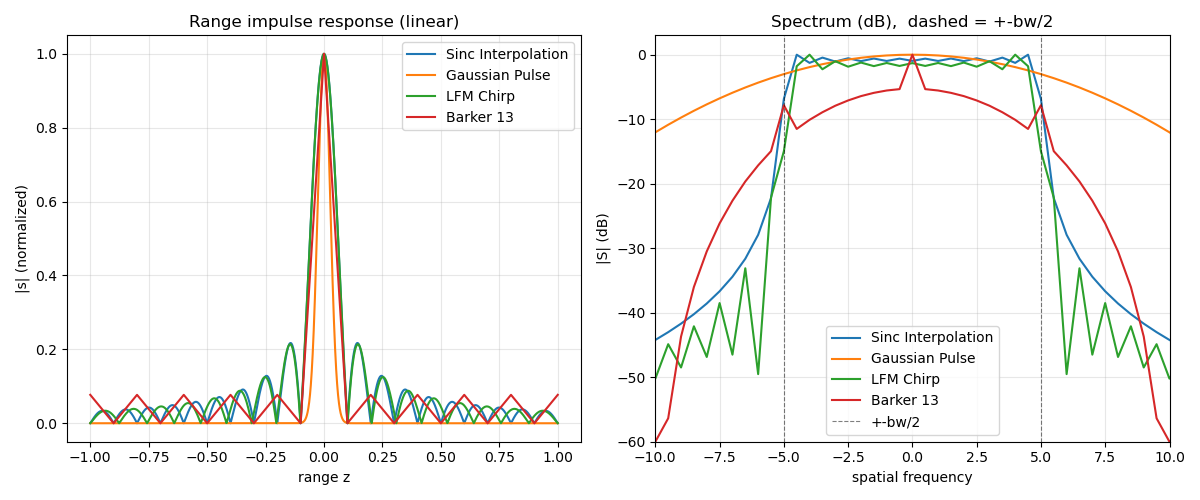
\includegraphics[width=\linewidth]{figs/window_analysis_bw10_fs2000.png}
  \caption{Effective interposummation windows $w(z) = h(z) * x(z)$ for a sinc, Gaussian, LFM chirp, and Barker-13 transmit waveform, all with spatial bandwidth $B_s = 10$. Left: range impulse response (linear, normalized). Right: spectrum in dB, with dashed lines marking $\pm B_s/2$.}
  \label{fig:effective-windows}
\end{figure}



\section{Experiments}
\label{sec:experiments}
We test our signal simulation with spotlight-mode SAR as described in the Jakowatz book \cite{spotlightmodesar}. The sensor is placed on the bottom side of every image, so illumination always arrives from that direction. Unless specified otherwise, all experiments use the default parameters shown in Table \ref{tab:params}. All results in this section are on the car model from the ShapeNet \cite{shapenet} cars dataset shown in Figure \ref{fig:main-fig}.a.
\begin{table}[h!]
\centering
\caption{Default experiment parameters, matching the \texttt{PAPER\_BASELINE} in \texttt{paper\_figures.py}.}
\label{tab:params}
\begin{tabular}{lll}
\toprule
\textbf{Symbol} & \textbf{Code variable} & \textbf{Default value} \\
\midrule
$P$                       & num\_pulse             & $64$ \\
$\Delta a$            & azimuth\_spread        & $90^\circ$ \\
$B_s$                     & spatial\_bw            & $73$ \\
$F_s$                     & spatial\_fs            & $73$ \\
$\lambda$                 & wavelength             & $0.5$ \\
SNR                       & snr\_db                & $50$~dB \\
$\sigma^2$                & trajectory\_noise\_var & $0$ \\
$R_w$                     & n\_ray\_width          & $128$ \\
$R_h$                     & n\_ray\_height         & $128$ \\
$W_g$                     & grid\_width            & $1.2$ \\
$H_g$                     & grid\_height           & $1.2$ \\
$(R,A,I,D,S)_{\text{obj}}$ & obj\_raids            & $(0.8, 0.0, 0.9, 0.1, 0.2)$ \\
$(R,A,I,D,S)_{\text{gnd}}$ & ground\_raids         & $(0.5, 0.0, 0.8, 0.2, 0.5)$ \\
\multicolumn{1}{c}{--} & num\_bounce            & $2$ \\
\multicolumn{1}{c}{--} & image\_width           & $128$ \\
\multicolumn{1}{c}{--} & image\_height          & $128$ \\
\multicolumn{1}{c}{--} & image\_plane\_width    & $1$ \\
\multicolumn{1}{c}{--} & image\_plane\_height   & $1$ \\
\multicolumn{1}{c}{--} & region\_radius         & $1.7$ \\
\multicolumn{1}{c}{--} & trajectory\_type       & circular \\
\multicolumn{1}{c}{--} & imaging\_algorithm     & cbp \\
\multicolumn{1}{c}{--} & cbp\_batch\_size       & $4096$ \\
\multicolumn{1}{c}{--} & use\_sig\_magnitude    & False \\
\multicolumn{1}{c}{--} & object\_x\_flip        & False \\
\multicolumn{1}{c}{--} & object\_rotate\_xyz    & $(90^\circ, 0^\circ, 0^\circ)$ \\
\bottomrule
\end{tabular}
\end{table}

In Figure \ref{fig:az-spread} we showcase our simulation when the range of azimuth angles (azimuth spread) is varied for the spotlight-mode SAR algorithm. With little azimuth spread, there is not much detail in the SAR image. At a $360^\circ$ spread the entire car is surrounded by the aperture, and a second set of fainter lines appears within the outline of the car due to the second bounce of the rays.
        
\begin{figure}
  \centering
  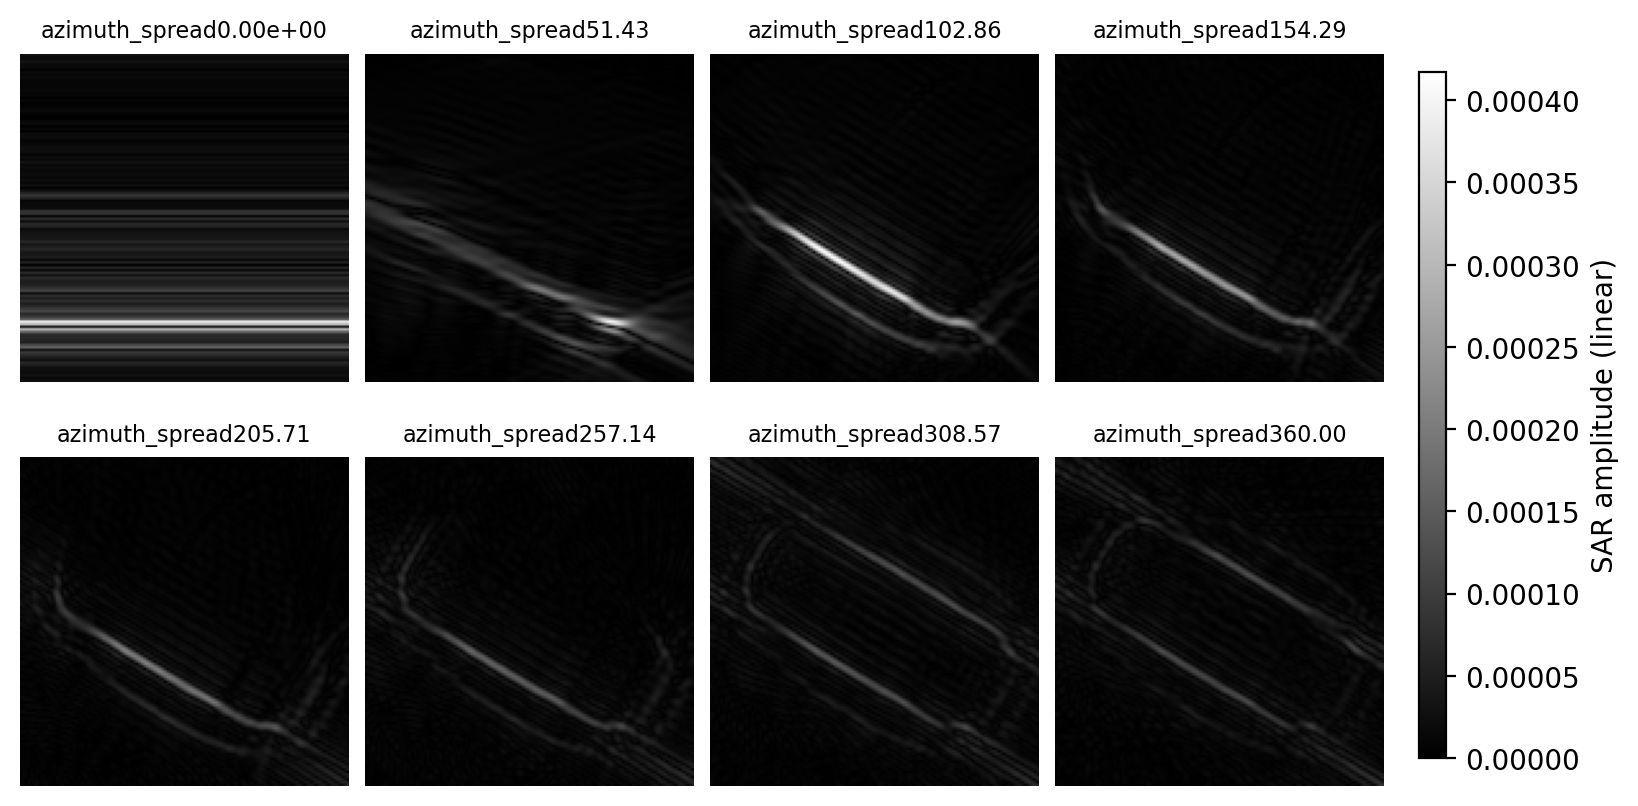
\includegraphics[trim=0 0 0 0, clip, width=0.48\textwidth]{figs/sar_stitched_az_spread.png}
  \caption{Varying the azimuth spread in our simulation.}
  \label{fig:az-spread}
\end{figure}

In Figure \ref{fig:num-pulse}, we illustrate the effect of varying the number of transmitted pulses in our simulation. With a small number of pulses, the reconstructed image appears coarse and lacks definition. As the pulse count increases, the image quality improves noticeably, revealing sharper boundaries and more distinct structural features of the target.
        
\begin{figure}
  \centering
  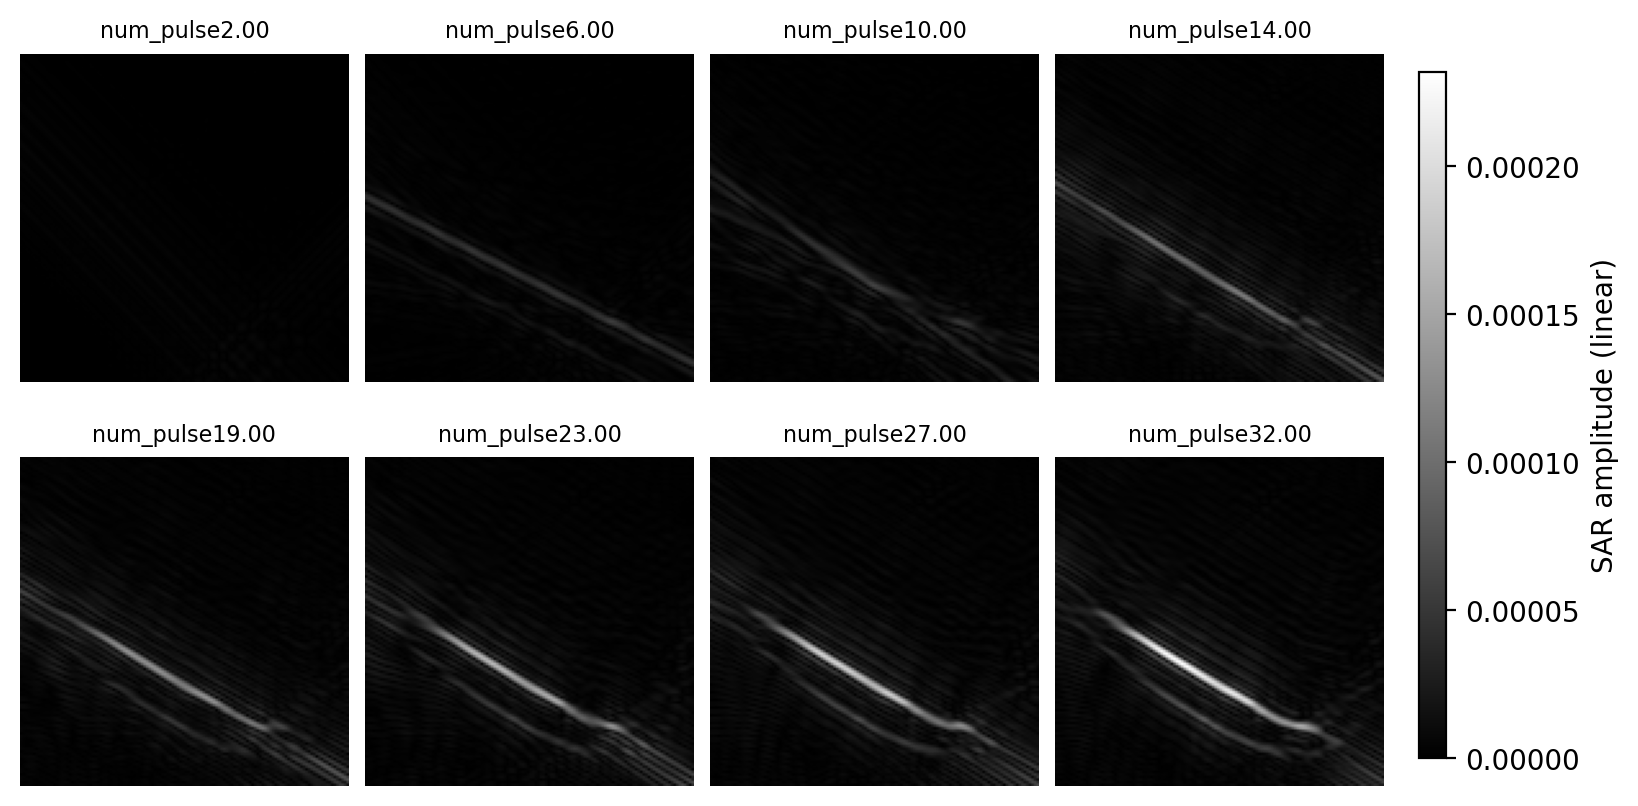
\includegraphics[trim=0 0 0 0, clip, width=0.48\textwidth]{figs/sar_stitched_num_pulse.png}
  \caption{Effect of varying the number of pulses in our simulation.}
  \label{fig:num-pulse}
\end{figure}

In Figure \ref{fig:snr}, we demonstrate how varying the signal-to-noise ratio (SNR) in decibels (dB) influences the quality of the simulated SAR image. In real SAR scenarios SNR decreases as range to the target increases. At low SNR values (around 0 dB), the image is dominated by noise, obscuring most structural details. As the SNR increases toward 22 dB, the object becomes clearly resolved, with well-defined features. SNR is calculated as an average over all signals used to generate the spotlight-mode SAR image.
        
\begin{figure}
  \centering
  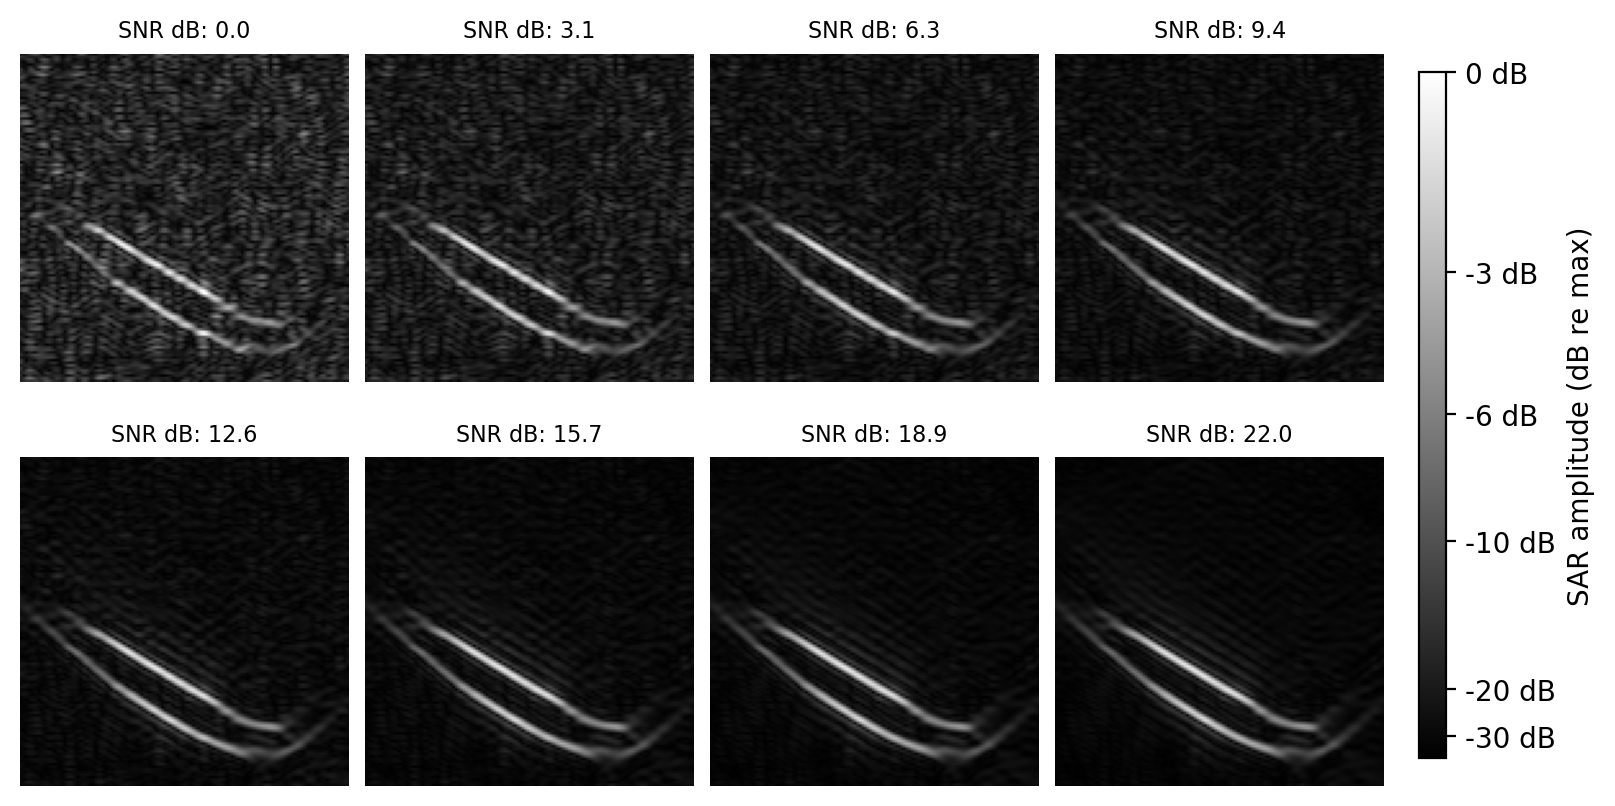
\includegraphics[trim=0 0 0 0, clip, width=0.48\textwidth]{figs/sar_stitched_snrdb.png}
  \caption{Varying the SNR in our simulation.}
  \label{fig:snr}
\end{figure}

In Figure \ref{fig:wavelength}, we analyze the effect of varying the wavelength parameter on the spotlight-mode SAR reconstruction. We use coherent integration of the complex-valued signals in both spotlight-mode and stripmap-mode SAR. Image quality is clearest at wavelengths that are well matched to the range resolution of the simulated system; wavelengths that are much shorter than the ray-grid spacing introduce interference patterns from constructive and destructive summation across nearby rays.

\begin{figure}[h!]
  \centering
  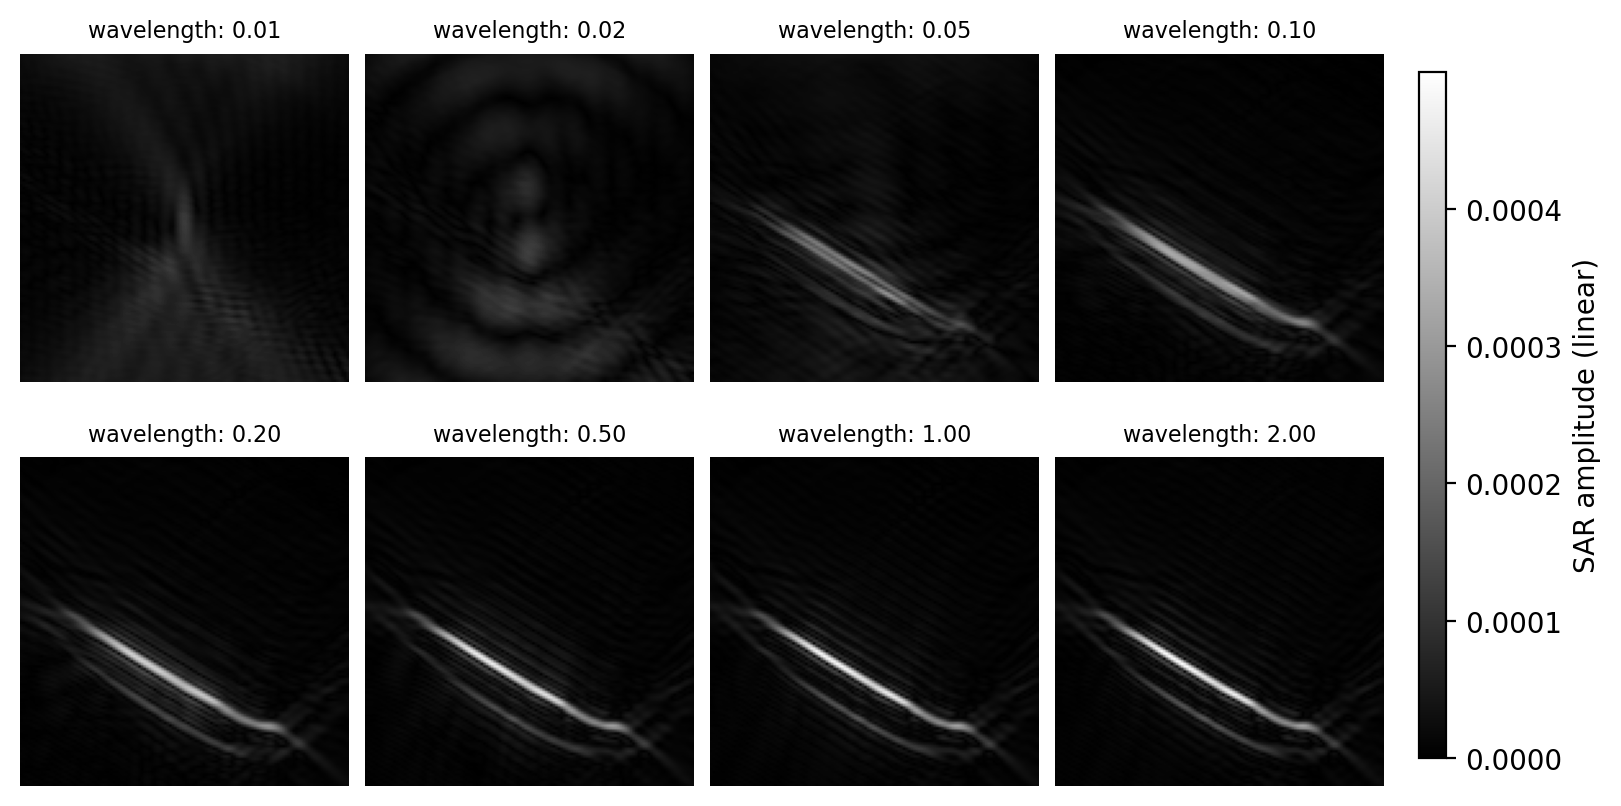
\includegraphics[trim=0 0 0 0, clip, width=0.48\textwidth]{figs/sar_stitched_wavelength.png}
  \caption{Varying the wavelength in our simulation with coherent integration.}
  \label{fig:wavelength}
\end{figure}

\subsection{Transmit Waveform}

In Figure \ref{fig:waveform}, we vary the transmit waveform, which replaces the
ideal sinc of interposummation with the effective window $w(z)$ of the
corresponding pulse-compression matched filter as described in Section
\ref{sec:method} and illustrated in Figure \ref{fig:effective-windows}. We
compare an ideal sinc, a Gaussian pulse, an LFM chirp, and a Barker-13 phase
code, all designed for the same spatial bandwidth $B_s$. The sinc, LFM chirp,
and Barker-13 reconstructions share a comparable range resolution but are
accompanied by the range sidelobes characteristic of each waveform, which
appear as faint replicas alongside the strong scatterers. The Gaussian pulse
produces no range sidelobes, but it does a poor job of suppressing
out-of-bandwidth frequencies, leaving much of its energy outside the allotted
band $\pm B_s/2$. Its gradual roll-off also tapers the in-band response, which
costs coherent gain and yields the visibly dimmer reconstruction in Figure
\ref{fig:waveform}.

\begin{figure}
  \centering
  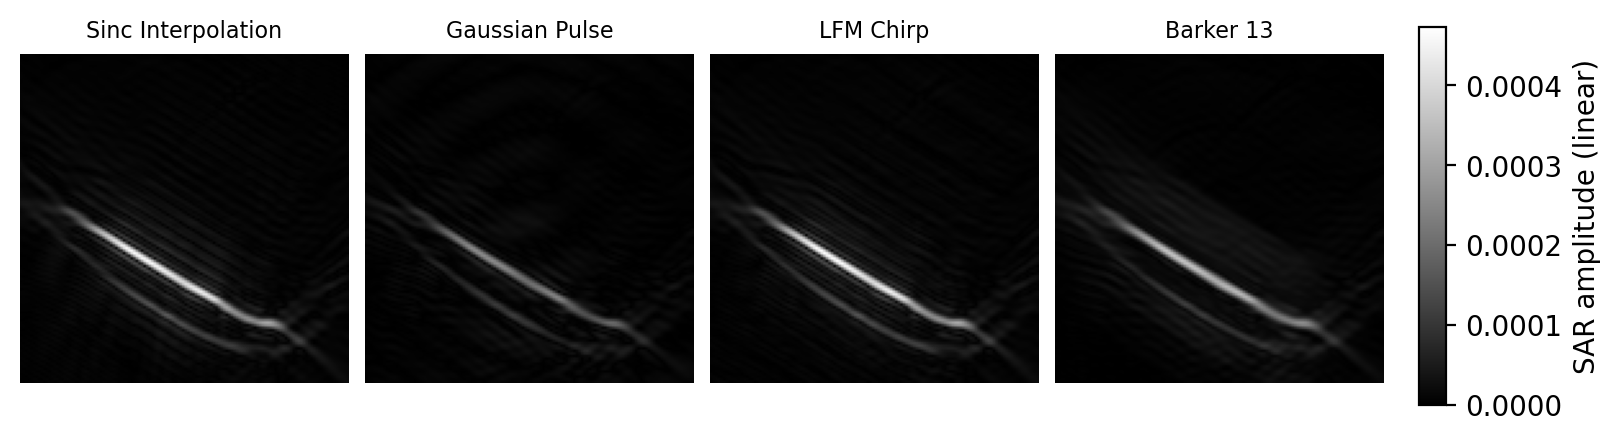
\includegraphics[trim=0 0 0 0, clip, width=0.48\textwidth]{figs/sar_stitched_waveform.png}
  \caption{Varying the transmit waveform in our simulation. Each panel uses the effective interposummation window $w(z)$ of the labeled pulse-compression waveform, all with the same spatial bandwidth $B_s$.}
  \label{fig:waveform}
\end{figure}

\subsection{Bandwidth and Ray Density}

In Figure \ref{fig:fsbw}, we analyze the effect of varying the spatial sample rate and bandwidth. Each plot indicates the sample rate in its caption, and we set the spatial bandwidth $B_s = F_s$ equal to the sampling frequency. The images are shown in dB scale with a shared DC maximum. As expected, the image resolution improves as both bandwidth and sample rate increase. However, an interesting artifact appears at $F_s = 512$, and to a lesser extent at $F_s = 256$. This occurs because, at high sampling rates, the discrete samples begin to capture the fine-scale variations of the continuous returned-signal model described in (\ref{eq:returned-scatters}). Since this signal model is composed of a series of delta functions, oversampling reveals its discontinuous nature rather than producing a smooth approximation, and the reconstructed SAR image degrades.

\begin{figure}
  \centering
  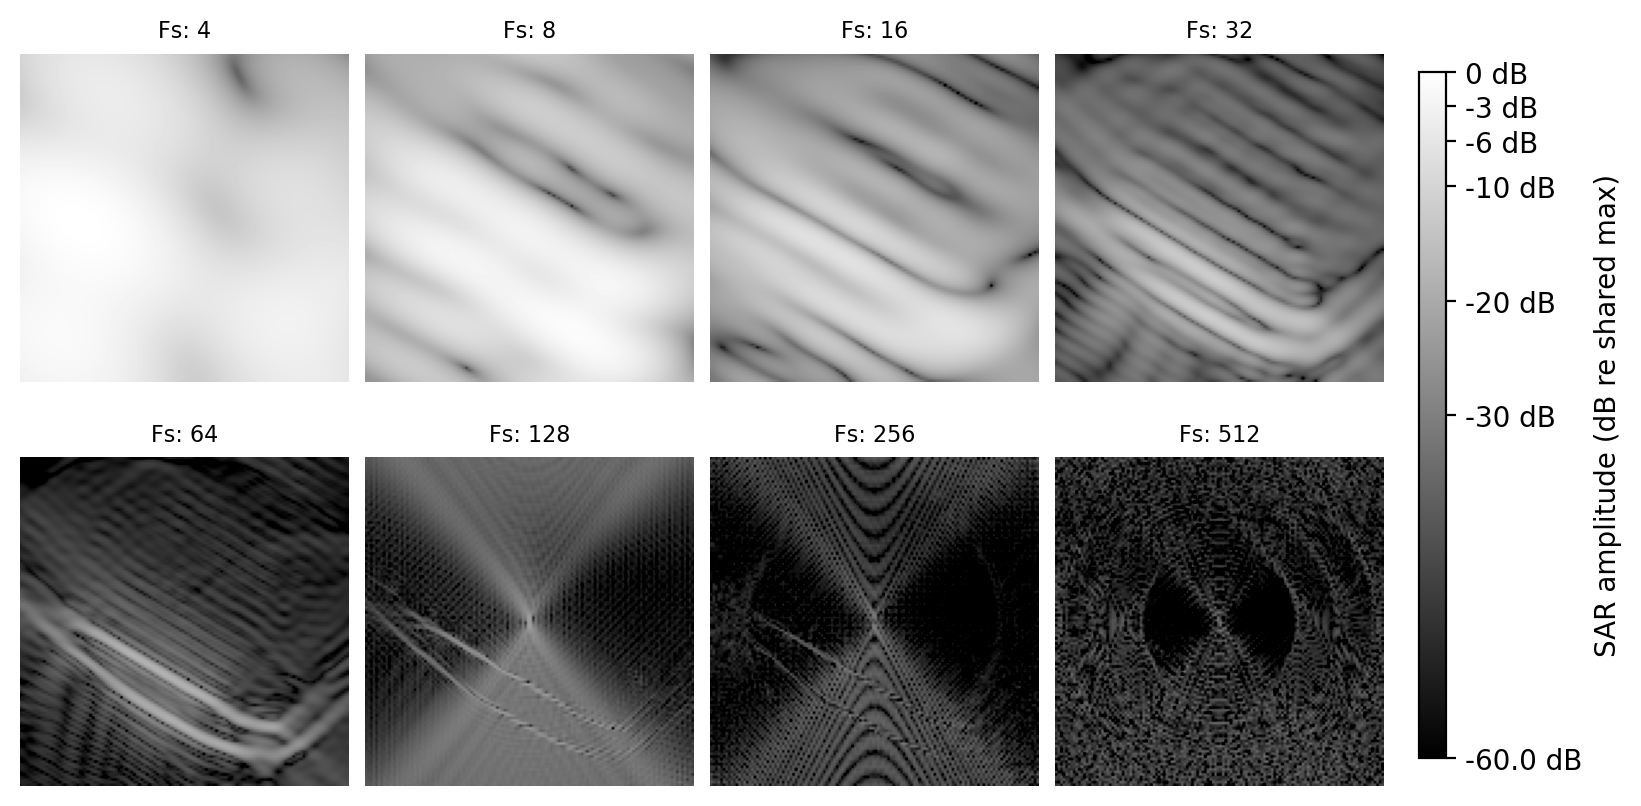
\includegraphics[trim=0 0 0 0, clip, width=0.48\textwidth]{figs/sar_stitched_fsbw.png}
  \caption{Varying the spatial sample rate and bandwidth in our simulation. Images are dB-scaled and share a common DC maximum.}
  \label{fig:fsbw}
\end{figure}

We further look into this problem in Figure \ref{fig:signals-square}. The figure presents the energy-range scatter plot (Figure \ref{fig:signals-square}.a) together with the corresponding interposummed signals at different bandwidth/sample rates (Figure \ref{fig:signals-square}.b-d). The signal appears clean at $F_s = B_s = 128$, whereas increasing the sampling rate and bandwidth to $256$ and $512$ results in the emergence of distinct artifacts from the Dirac delta functions as described in (\ref{eq:returned-scatters}).
\begin{figure}[t]
    \centering
    % First row
    \begin{subfigure}[b]{0.48\columnwidth}
        \centering
        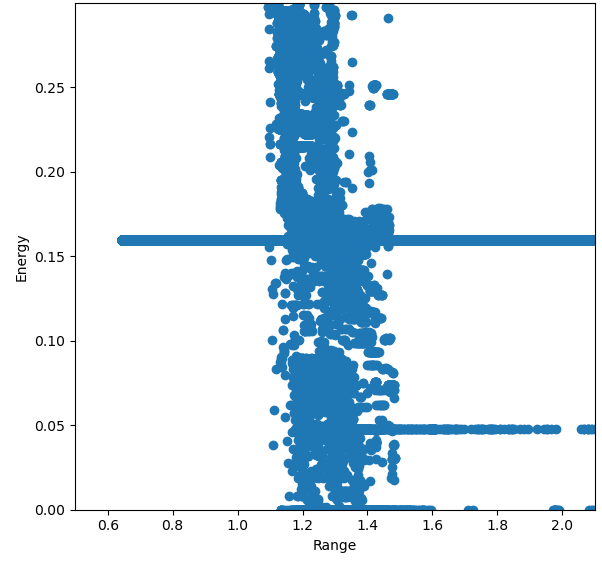
\includegraphics[width=\linewidth]{figs/scatters.png}
        \caption{}
        \label{fig:scatters}
    \end{subfigure}
    \hfill
    \begin{subfigure}[b]{0.48\columnwidth}
        \centering
        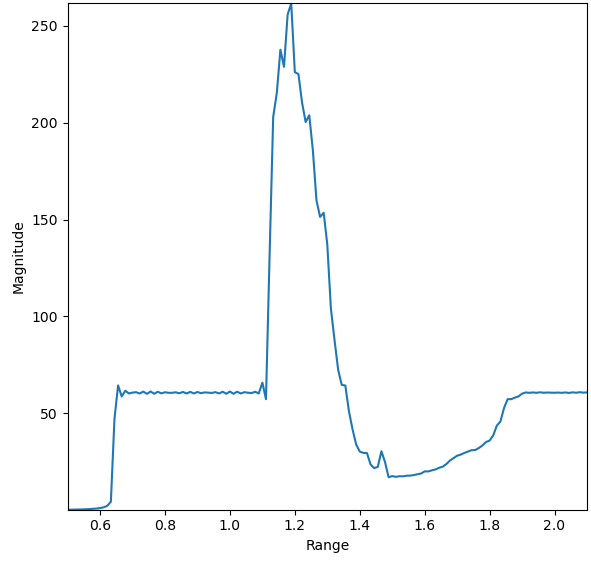
\includegraphics[width=\linewidth]{figs/signal_clean.png}
        \caption{}
        \label{fig:signal-clean}
    \end{subfigure}

    % Small vertical space
    \vspace{0.3em}

    % Second row
    \begin{subfigure}[b]{0.48\columnwidth}
        \centering
        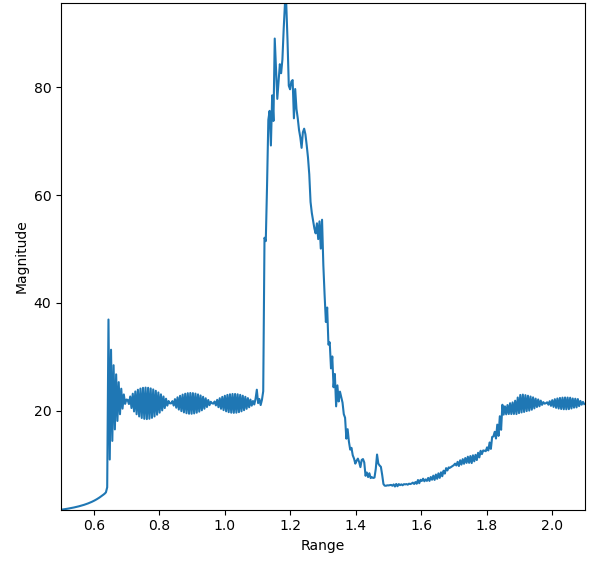
\includegraphics[width=\linewidth]{figs/signal_dirty.png}
        \caption{}
        \label{fig:signal-dirty}
    \end{subfigure}
    \hfill
    \begin{subfigure}[b]{0.48\columnwidth}
        \centering
        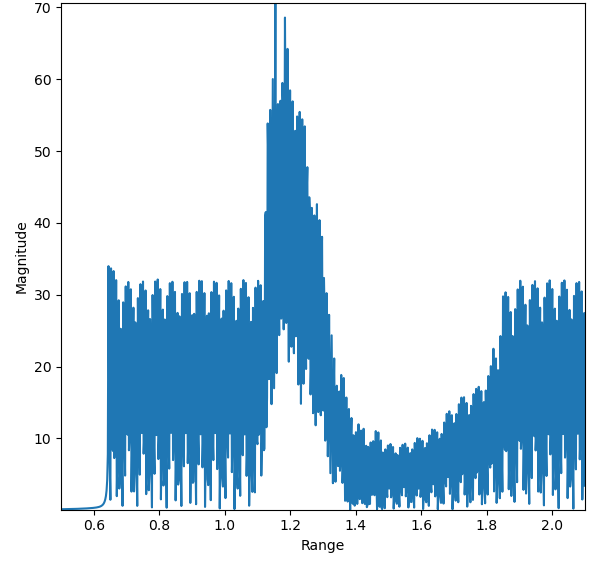
\includegraphics[width=\linewidth]{figs/signal_nasty.png}
        \caption{}
        \label{fig:signal-nasty}
    \end{subfigure}

    \caption{Comparison of the energy-range scatter (a), and the signal at an $F_s=B_s$ of 128 (b), 256 (c), and 512 (d). Oversampling the energy-range scatter results in a jagged signal.}
    \label{fig:signals-square}
\end{figure}

There are two ways to mitigate this effect: increasing the number of rays $(R_h, R_w)$, and decreasing the spatial bandwidth $B_s$. A denser ray grid allows for more scatters near the center of the sinc pulses in interposummation, which reduces the variable sums between neighboring sincs. Decreasing the spatial bandwidth $B_s$ of the interposummation accomplishes the same goal, but by widening the sinc pulses to accumulate more scatters instead of adding more scatters. The trade-offs between the two solutions are that increasing the ray density increases the computational complexity, and decreasing the bandwidth reduces image quality.

\subsection{Sensor Trajectory}

In Figure \ref{fig:trajectory-type}, we compare the two supported sensor trajectories. The circular trajectory sweeps the sensor along a constant-radius arc around the target, while the linear trajectory translates the sensor along a straight path. The circular trajectory produces a more uniformly illuminated image because the range from the sensor to the target is nearly constant across pulses.

\begin{figure}
  \centering
  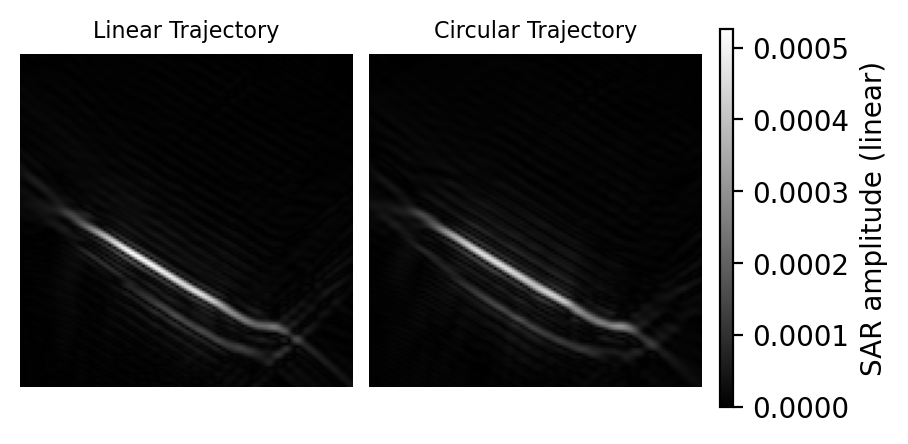
\includegraphics[trim=0 0 0 0, clip, width=0.34\textwidth]{figs/sar_stitched_trajectory_type.png}
  \caption{Comparison of circular and linear sensor trajectories in our simulation.}
  \label{fig:trajectory-type}
\end{figure}

In Figure \ref{fig:trajectory-noise}, we analyze the impact of imperfect knowledge of the sensor trajectory. We add zero-mean Gaussian noise with variance $\sigma^2$ to the perceived sensor position while the true trajectory used for signal simulation is kept noise-free. This models the case where the reconstruction algorithm has an imprecise estimate of the sensor pose. As the noise variance increases, the reconstructed image becomes progressively blurred as the pulses no longer coherently integrate at the correct locations.

\begin{figure}
  \centering
  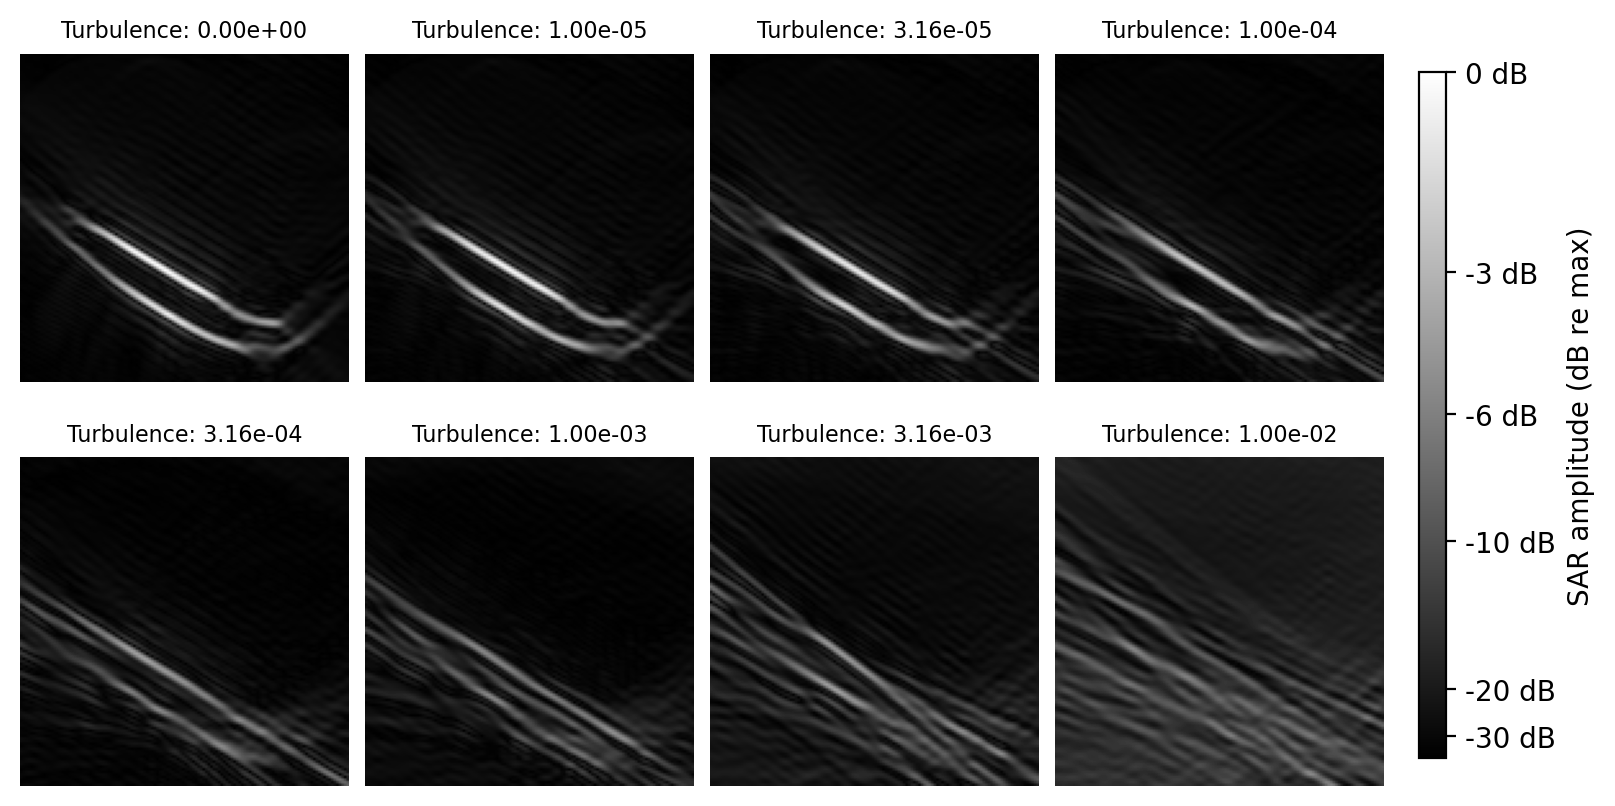
\includegraphics[trim=0 0 0 0, clip, width=0.48\textwidth]{figs/sar_stitched_trajectory_noise_var.png}
  \caption{Effect of trajectory position noise variance on the reconstructed SAR image.}
  \label{fig:trajectory-noise}
\end{figure}

\subsection{Sphere Rendering}

In Figure \ref{fig:sphere-size}, we render a sphere at five successively halved scales ($1$, $1/2$, $1/4$, $1/8$, and $1/16$ of the mesh's native size), with the ground plane removed and the pulse count raised to $256$ to resolve the smaller targets. As the sphere shrinks, its return contracts toward the image center while preserving the curved signature of the illuminated surface. The curve of this signature tightens as the scale decreases, and at the smallest scales the return collapses toward a compact response resembling that of a point scatterer. The sidelobes of the response appear in all directions around the target: because the sphere backscatters equally from every observable angle, the sidelobe energy is distributed symmetrically, producing the concentric ring pattern visible around each target.

\begin{figure}
  \centering
  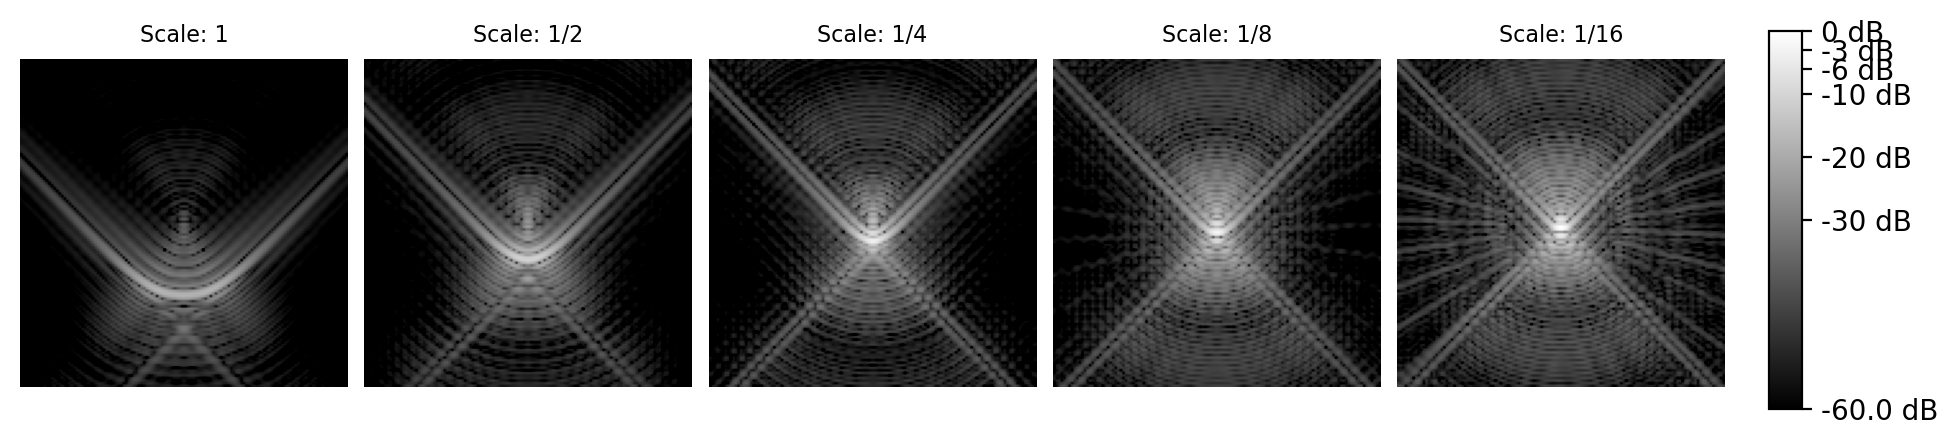
\includegraphics[trim=0 0 0 0, clip, width=0.48\textwidth]{figs/sar_stitched_sphere_size.png}
  \caption{SAR reconstruction of a sphere at decreasing scale, shown in dB, with the scale factor labeled above each subplot.}
  \label{fig:sphere-size}
\end{figure}

\section{Conclusion}
\label{sec:conclusion}
In this paper, we presented an open-source, GPU-accelerated SAR simulator implemented in PyTorch
that supports arbitrary 3D \texttt{.obj} models, multi-bounce ray tracing, and configurable radar
parameters such as wavelength, bandwidth, sample rate, and material properties. It addresses the
limitations of existing open-source tools such as \emph{RaySAR} and \emph{CVDomes}, which are
constrained in mode support and rely on outdated software such as MATLAB.

The proposed \emph{interposummation} technique enables efficient low-pass filtering during the
summation and interpolation of ray returns, accounting for the radar system's bandwidth and
sampling rate. This allows the simulator to generate physically meaningful signals without
aliasing or distortion due to improper interpolation.

We conducted a series of experiments using spotlight-mode SAR simulations over ShapeNet car models
while varying key parameters such as radar bandwidth, wavelength, and sampling rate. These
experiments demonstrate how system parameters influence image quality and signal fidelity. In
particular, we observed that excessive oversampling of the energy-range scatter leads to poor
signal quality and numerical artifacts. This can be mitigated either by reducing the effective
bandwidth, which lowers the required sampling rate, or by increasing the ray density to maintain
consistent energy coverage across the target surface.
Future work will extend the simulator to support arbitrary flight paths, synthetic aperture SONAR,
and simulations that include jamming, broadening its applicability to a wider set of radar and
sonar scenarios.




%%%%%%%%% REFERENCES
{\small
\bibliographystyle{ieee_fullname}
\bibliography{egbib}
}

\end{document}
